\section{Introduction}
Seasonal tropical cyclone (TC) forecasting has become an active field of research \cite{elsner1993, elsner1998, elsner2008, klotzbach2009}. While seasonal forecasts cannot inform the frequency or intensity of landfalling hurricanes, aggregate TC statistics such as counts are regarded as valuable by the reinsurance industry and are useful for forecasting the environment's response to seasonal TC activity -- for example ocean heat transport or phytoplankton blooms. A primary driver of seasonal TC activity are the large-scale conditions over the Atlantic basin and any reasonable attempt at skillful seasonal prediction should be able to reproduce these conditions \cite{gray1968}, even if synoptic-scale (\emph{i.e.} African Easterly Waves, \emph{etc.}) and stochastic events cannot be accounted for \cite{Knutson2007, Emanuel2008Simulation}.

One of the well-documented influencers of Atlantic TC activity on seasonal timescales through large-scale conditions is the El-Ni\~no Southern Oscillation (ENSO): the quasi-periodic cycle of warming and cooling of the near equatorial Pacific sea surface temperatures (SST). Some of the earliest empirical studies proposed that enhanced convection as a result of anomalous Eastern Pacific Ocean warming is associated with strong westerly upper tropospheric wind over the Caribbean basin and tropical Atlantic, resulting in low TC activity during ENSO's warm phase (El Ni\~no) and high TC activity during its cold phase (La Ni\~na) \cite{gray1984a}. Other studies have suggested that ENSO influences Atlantic TC activity via tropospheric warming \cite{tang2004}. Hwoever, a closer examination of the number of TCs on a seasonal-scale as a function of ENSO's phase 

For the past 50 years, numerous attempts to represent such a cycle using empirical warming-based indices have been made. Indices such as NINO1+2 and NINO3.4 are constructed by averaging the sea surface temperature (SST) anomalies of static oceanic regions and are subsequently related to Atlantic TC activity \cite{trenberth1997definition}. While such indices have been a staple of long-range teleconnection research, recent studies suggest that to fully capture ENSO activity, it is no longer sufficient to monitor the warm and cold phases of the Eastern Pacific. Some research proposes to monitor several regions concurrently \cite{trenberth2001,ren2011} or focus on the Central Pacific \cite{ashok2007}. Warming in the Central Pacific, known as El Ni\~no Modoki (or Central Pacific ENSO), where warm waters are surrounded by cold ones has been observed with increased frequency since the 1990s. Such changes have been attributed to anthropogenic global warming \cite{yeh2009} as well as natural climate variability \cite{wittenberg2009} and might affect Atlantic TC landfalling probabilities \cite{kim2009}. 


%Given the increasing number of studies reporting a shift in the spatial warming patterns of the Pacific it comes as surprise that monitoring static East Pacific regions is less informative of Atlantic TC activity (see Figure \ref{fig:figures_nino_tc_bars}). 


 


%the equatorial Pacific Ocean experiences weak easterly winds causing an increase in Eastern Pacific SSTs, that in turn alters the atmospheric zonal (Walker) circulation, generally resulting in prevailing westerlies. ENSO's cold, La Ni\~na (LN) phase, is characterized by the opposite atmospheric conditions -- with cold SST anomalies along the Eastern Pacific and warm ones near the Western Pacific as a result of prevailing easterly winds.  % (see Figure \ref{fig:enso_cartoon}). The mechanisms that control the reversal to the opposite LN phase are not fully understood \cite{kirtman1997,smith2012}. 



\begin{figure}[htbp]
	\centering
		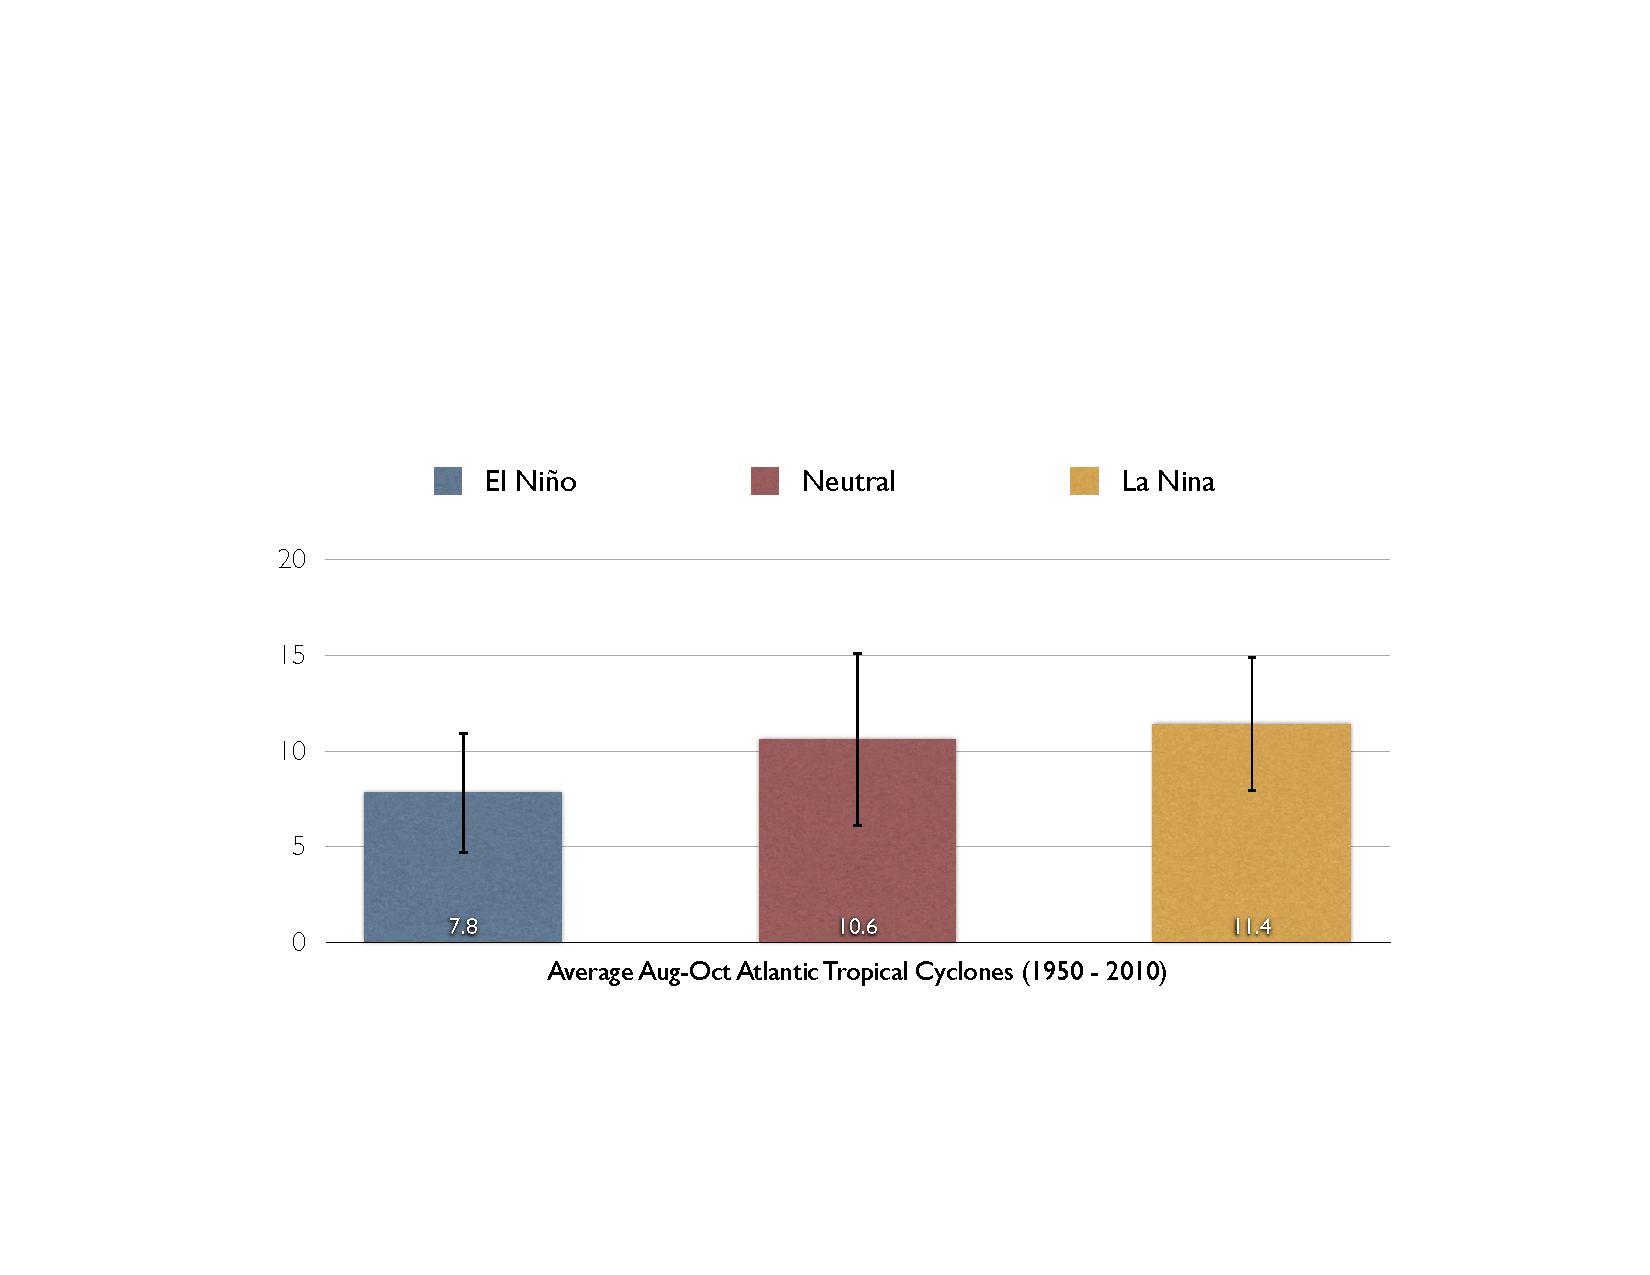
\includegraphics[height=3in]{figures/nino_tc_bars.pdf}
	\caption{The mean August-October Atlantic TC counts. Error bars denote one standard deviation. This figure shows that while there are notable differences in TC counts based on the phase of ENSO, the large variability of TC counts make discerning ENSO's impact uncertain. The NINO3.4 index was built using ERSSTV3. TC counts are from the Unisys best track archive.}
	\label{fig:figures_nino_tc_bars}
\end{figure}

Given that ENSO affects the large-scale conditions over the Atlantic through anomalous warming and its associated wind shear, it is not only important to monitor the intensity of warming along the equatorial Pacific -- something traditional NINO indices do -- but also to capture the location of the warming. We propose a distance-based ENSO index (S-ENSO for spatial ENSO) that tracks the longitude of highest SST anomaly in the tropical Pacific. We demonstrate its robustness in predicting seasonal Atlantic TC activity as well as resolving the large-scale conditions over the Atlantic. Such an index, coupled with other seasonal prediction methods based on Atlantic variables (e.g. \cite{knutson2007, emanuel2008simulation}) may prove to be a significant addition to dynamical and statistical TC forecast models.

\newpage

% 

%an increasing number of studies report a shifting in the spatial warming patterns of the Pacific therefore making the monitoring of fixed regions less informative (see Figure 1). 


%A common pathway by which Pacific SST warming affects the globe is through the alteration of the Walker circulation due to ---. 


%are Pacific sea surface temperatures (SST). Traditionally, Pacific SST's impact of the Atlantic has been abstracted by monitoring the warming of fixed oceanic regions (e.g. NINO3.4). However increasing evidence is suggesting that the spatio-temporal context of the warming must be considered (relative SST, NINO Modoki, etc.)

%We propose a new index that accounts for the spatial distribution of warming of Pacific SSTs and are able to explain 60\% of the seasonal variability in Atlantic TC frequency. The index is able to resolve the large-scale conditions during the Atlantic hurricane season better than warming-based indices. Such an index, coupled with other seasonal prediction methods based on Atlantic variables (e.g. Kneuston et al 2007, Emanuel et al 2008) can prove to be a significant addition to dynamical and statistical forecast models.

%A second approach to the problem is to use statistical relationships between tropical cyclones and large-scale predictors to estimate tropical cyclone activity as a function of variables that are resolved by climate models (e.g., Camargo et al. 2007a,b). One potential drawback of this approach is that the statistics are trained largely on natural variability, much of which is regional; it is not clear that such indices will perform well when applied to global climate change

% Pacific Ocean sea surface temperatures (SSTs) have well documented global long-range teleconnections, including Atlantic tropical cyclone (TC) activity \cite{gray1984a, bove1998,elsner2001b, emanuel2008, klotzbach2011nino}. The quasi-periodic cycle (2-7 years) of warming and cooling of the near equatorial Pacific Ocean, known as the El-Ni\~no Southern Oscillation (ENSO), has been used to predict Atlantic TC activity for decades. However, due to the large amplitude variations in seasonal TC counts, the difference in Atlantic TC activity based on the phase of ENSO is not obvious (see Figure \ref{fig:enso_bars}).
% 
% Traditionally, ENSO has been quantified using warming-based indices where SST anomalies are averaged over fixed regions in the Pacific Ocean. An increasing number of studies suggest that monitoring static regions may not be enough to capture the complex ENSO phenomenon \cite{trenberth2001, ashok2007,yeh2009,kim2009}. Furthermore, other studies proposed that the Pacific Ocean warming patterns are changing - with warm anomalies shifting towards the Central Pacific. Such changes have been attributed to anthropogenic global warming \cite{yeh2009} as well as natural climate variability \cite{wittenberg2009}. Based on these findings, it is evident that in order to capture ENSO's long range impact on the tropical Atlantic a new measure of Pacific warming is needed. 
% 
% 
% 
% We propose a novel spatial ENSO index (S-ENSO) that is designed specifically to capture the physical pathways by which Pacific SSTs may influence Atlantic TC activity. Tropical Atlantic SST variability west of 40W and extending into the Caribbean is correlated with Pacific ENSO variability, with 50-80\% of the anomalous SST variability in the region associated with ENSO \cite{enfield97}. However, a large number of TCs, especially the most intense hurricanes, originate east of 40W (based on the NOAA best track hurricane data). Therefore, it is important for any index to resolve the large-scale conditions over the eastern tropical Atlantic. Our approach introduces a distance-based ENSO index that tracks the location of maximum near-tropical Pacific warming anomaly instead of its absolute warming. We will demonstrate the performance of our index by comparing it to traditional warming-based ENSO indices in discriminating between the large-scale conditions that are favorable for Atlantic cyclogenesis.
